\documentclass[conference]{IEEEtran}
\IEEEoverridecommandlockouts

\usepackage[T1]{fontenc}
\usepackage{lmodern}
\usepackage{cite}
\usepackage{amsmath,amssymb,amsfonts}
\newcommand{\mathds}[1]{\mathbf{#1}}
\usepackage{algorithmic}
\usepackage{graphicx}
\usepackage{textcomp}
\usepackage{xcolor}
\usepackage{booktabs}
\usepackage{hyperref}

\def\BibTeX{{\rm B\kern-.05em{\sc i\kern-.025em b}\kern-.08em
    T\kern-.1667em\lower.7ex\hbox{E}\kern-.125emX}}

\begin{document}

\title{Adaptive Stress Testing for Algorithmic Trading: \\An Importance Sampling Approach}

\author{\IEEEauthorblockN{Esaw Adhana}
\IEEEauthorblockA{\textit{CS 238V: Validation of Autonomous Systems} \\
Stanford University \\
esawadhana@stanford.edu}}

\maketitle

% ============================================================
\begin{abstract}
Validating the safety of algorithmic trading strategies is challenging because
catastrophic failure events, such large, rapid "drawdowns" are rare under normal market conditions, making naïve Monte Carlo (MC) sampling computationally expensive. We apply Adaptive Stress Testing (AST), a reinforcement learning
framework that trains an adversarial agent to efficiently discover worst-case
failure trajectories in a target system. We evaluate AST against a Simple Moving Average (SMA) crossover trading strategy in a simulated market environment across two victim configurations: a baseline strategy (V1, with 5-step exit lag) and a more robust strategy (V2, 3-step exit lag).
An adversarial Proximal Policy Optimization (PPO) agent is trained against each victim, and importance sampling (IS) is used to translate the biased adversarial failure trajectories
into unbiased estimates of the real-world failure probability under the
nominal market distribution.
Our results (mean $\pm$ std over 5 evaluation trials) show that AST achieves
$100.0 \pm 0.0\%$ failure rate against V1 compared to only $0.4 \pm 0.3\%$
for MC, a $\geq\!250\times$ improvement in failure discovery, while the IS
estimate reveals these failures have probability
$\approx 1.5 \times 10^{-11}$ under natural market noise.
Against V2, an adversary trained with twice the compute budget (400k vs.\ 200k timesteps)
achieves only $62.0 \pm 2.6\%$ failure, with IS-estimated probability
$2.0 \times 10^{-3}$, more than eight orders of magnitude higher, revealing
that V2's failures, though harder to find, are far more realistic.
These results expose a critical insight, namely that raw failure rate is a deceptive
safety metric. V1 appears more dangerous by failure rate ($100.0\%$ vs.\
$62.0\%$), yet IS reveals V2's failures are more than eight orders of
magnitude more likely under natural market conditions. The combination of
adversarial sample complexity and IS-corrected failure probability, not merely failure rate,
provides the full picture of safety.
\end{abstract}

\begin{IEEEkeywords}
adaptive stress testing, algorithmic trading, safety validation,
reinforcement learning, importance sampling, failure probability estimation
\end{IEEEkeywords}

% ============================================================
\section{Introduction}

The deployment of automated algorithmic trading systems in real financial
markets raises fundamental safety questions: Under what market conditions
might the system suffer a catastrophic loss, and how likely are such conditions
to occur? Answering these questions is difficult because catastrophic failure
events, such as a portfolio losing a majority of its value within minutes, are
rare under typical market dynamics. Traditional validation approaches
based on Monte Carlo simulation are statistically inefficient for rare-event
estimation, requiring an exponentially large number of samples to reliably
observe even a single failure.

Adaptive Stress Testing (AST)~\cite{lee2015adaptive,koren2018adaptive,lee2020adaptive} addresses this
inefficiency by framing the failure-finding problem as a Markov Decision
Process (MDP) in which a learned adversarial agent controls the stochastic
inputs to the system under test. The adversary is trained via reinforcement
learning (RL) to maximize the probability of inducing failures, effectively
acting as an importance-weighted sampler over the space of failure-inducing
trajectories.

In this work, we apply AST to validate two versions of a simulated SMA
crossover trading strategy, which represents a widely deployed class of
technical analysis algorithms. We make the following implementation contributions:

\begin{enumerate}
  \item We construct a Gymnasium simulation environment that models an
    adversarial stochastic market and two victim trading strategy variants
    (V1 and V2, with 5-step and 3-step exit lags, respectively, where the exit lag represents the number of consecutive bearish steps required before the position is liquidated).
  \item We train PPO-based adversaries against each victim and compare
    failure discovery efficiency against a Monte Carlo baseline.
  \item We implement importance sampling to estimate the real-world probability
    of failure under the nominal $\mathcal{N}(0,1)$ market distribution.
  \item We demonstrate that iterative adversarial robustness improvement (reducing
    the exit lag from 5 to 3 steps between V1 and V2) substantially increases adversarial
    sample complexity: against V2, even doubling the training budget (400k vs.\ 200k timesteps)
    yields only $62.0 \pm 2.6\%$ failure rate versus $100.0\%$ for V1, while IS
    reveals V2's residual failures are more than eight orders of magnitude
    more realistic.
\end{enumerate}

% ============================================================
\section{Related Work}

\subsection{Adaptive Stress Testing}
AST was originally introduced by Lee et al.~\cite{lee2015adaptive} as a
method for finding the most likely failure scenarios in black-box systems,
initially applied to aircraft collision avoidance using Monte Carlo Tree
Search (MCTS). Subsequent work by Koren et al.~\cite{koren2018adaptive}
extended the AST framework to autonomous vehicles and introduced Deep
Reinforcement Learning (DRL) policies as a highly scalable alternative to
MCTS. The generalized AST framework, encompassing both MCTS and deep RL
approaches, is formally detailed in~\cite{lee2020adaptive}.

\subsection{Rare-Event Estimation via Importance Sampling}
Importance sampling (IS) is a variance-reduction technique for
estimating expectations under a target distribution by sampling from a
different, more convenient proposal distribution~\cite{tokdar2010is}.
In the context of safety validation, IS has been used to convert failure
trajectories found under a biased search distribution back into
probability estimates under the nominal environment
distribution~\cite{zhao2016accelerated}. The combination of AST with IS
was explored in~\cite{corso2021survey}, which surveys rare-event simulation
methods for autonomous system validation.

\subsection{Algorithmic Trading Safety}
Technical analysis strategies such as SMA crossovers are among the most
widely used systematic trading methods~\cite{brock1992sma}.
Robustness of such strategies to adversarial or anomalous market conditions
is studied in the context of flash crashes~\cite{kirilenko2017flash} and
adversarial market manipulation~\cite{brunnermeier2005predatory}.
Our work bridges safety validation methodology and algorithmic trading,
applying RL-based stress testing to estimate the probability of large
drawdown events.

% ============================================================
\section{Background}

\subsection{Importance Sampling for Failure Probability}

Let $\mathbf{x} \in \mathbb{R}^d$ be a vector of environmental disturbances drawn
from a nominal distribution $p_0(\mathbf{x})$ and let $f(\mathbf{x}) \leq 0$ denote
a failure event. The failure probability is
\begin{equation}
  P_F = \mathbb{E}_{p_0}\!\left[\mathbf{1}\{f(\mathbf{x}) \leq 0\}\right]
      = \int \mathbf{1}\{f(\mathbf{x}) \leq 0\}\, p_0(\mathbf{x})\, d\mathbf{x}.
\end{equation}
A naive Monte Carlo estimate $\hat{P}_F = \frac{1}{N}\sum_i \mathbf{1}\{f(\mathbf{x}_i)\leq 0\}$
has coefficient of variation $\sqrt{(1-P_F)/(N P_F)}$, which grows
without bound as $P_F \to 0$~\cite{tokdar2010is}.
Importance sampling (IS) draws from a proposal $q(\mathbf{x})$ that concentrates
mass near failures and corrects via likelihood ratios:
\begin{equation}
  \hat{P}_F^{\text{IS}} = \frac{1}{N}\sum_{i=1}^{N}
    \mathbf{1}\{f(\mathbf{x}_i)\leq 0\}\cdot\frac{p_0(\mathbf{x}_i)}{q(\mathbf{x}_i)},
    \quad \mathbf{x}_i \sim q.
\end{equation}
This estimate is unbiased and has substantially lower variance when $q$ is
concentrated in the failure region~\cite{corso2021survey}.

\subsection{Adaptive Stress Testing}

Adaptive Stress Testing (AST)~\cite{lee2015adaptive,koren2018adaptive,lee2020adaptive} frames failure-finding as
an MDP $\langle \mathcal{S}, \mathcal{A}, T, R, \gamma \rangle$ where
$\mathcal{S}$ is the joint system state, $\mathcal{A}$ is the space of
environmental disturbances the adversary injects at each step,
$T(s'\mid s,a)$ is the (black-box) system transition, and the reward
$R(s,a,s')$ is designed to maximize failure probability.
A reinforcement learning agent trained on this MDP learns a proposal policy
$\pi_\theta$ that acts as an importance-weighted sampler over failure-inducing
trajectories.  Trajectory-level IS weights
$w^{(i)} = \exp\!\bigl(\sum_t \log p_0(a_t) - \log \pi_\theta(a_t \mid s_t)\bigr)$
convert adversarial episodes into unbiased estimates of $P_F$ under $p_0$.

% ============================================================
\section{Methodology}

\subsection{Simulation Environment}

We implement a custom Gymnasium environment, \texttt{TradingValidationEnv},
in which an adversary injects per-step noise $\varepsilon_t$ into the
market's log-return. The asset price evolves as:
\begin{equation}
  p_{t+1} = p_t \left(1 + \mu + \sigma \varepsilon_t\right),
  \quad \varepsilon_t \sim \mathcal{N}(0,1) \text{ (nominal)},
\end{equation}
where $\mu = 0.0001$ is the drift and $\sigma = 0.02$ is the volatility
scale. The adversary's action space is $\varepsilon_t \in [-3, 3]$.

The five-dimensional observation at each step is:
\[
  s_t = \left[p_t,\; V_t,\; \text{SMA}_{50},\; \text{SMA}_{200},\; \mathds{1}_{\text{invested}}\right],
\]
where $\text{SMA}_{50}$ and $\text{SMA}_{200}$ are the 50-step and 200-step simple moving averages of the asset price, $V_t$ is the current portfolio value, and $\mathds{1}_{\text{invested}}$
is a flag indicating whether the victim strategy is currently holding the asset.

A \emph{failure} is defined as the portfolio value falling below $V_f = \$700$,
corresponding to a 30\% drawdown from the initial value of $\$1{,}000$.
Each episode runs for at most 100 steps.

\subsection{Victim Trading Strategies}

\textbf{Victim V1 (Baseline).}
V1 implements a standard SMA crossover strategy: the bot buys and holds
the asset when $\text{SMA}_{50} > \text{SMA}_{200}$ and exits when
$\text{SMA}_{50} \leq \text{SMA}_{200}$. To reflect realistic execution
latency, an \emph{exit lag} of 5 consecutive bearish steps is required
before the position is liquidated. This lag creates exploitable inertia:
the bot remains invested through the early phase of a crash.

\textbf{Victim V2 (More Robust).}
V2 uses the same SMA-50/200 crossover logic as V1 but reduces the exit lag
from 5 steps to 3. This directly addresses the exploit discovered in V1:
by requiring only 3 consecutive bearish SMA steps before selling (instead of
5), the bot limits the window of inertia the adversary can exploit. The
effect is an increase in \emph{adversarial sample complexity}: an adversary
trained for 200k timesteps exploits V1 trivially ($100.0\%$ failure), while
doubling the training budget to 400k timesteps against V2 still yields only
a $62.0 \pm 2.6\%$ failure rate, as shown in Table~\ref{tab:results}.

\subsection{Adversarial AST Agent}

The adversary is a Proximal Policy Optimization (PPO)~\cite{schulman2017ppo}
agent with an MLP policy (two hidden layers of 64 units each), implemented
using Stable-Baselines3~\cite{raffin2021sb3}. The reward signal is:
\begin{equation}
  r_t = \underbrace{\frac{V_{t-1} - V_t}{2}}_{\text{damage reward}}
       \underbrace{- 0.05\,\varepsilon_t^2}_{\text{likelihood penalty}}
       + \underbrace{1000 \cdot \mathds{1}_{[V_t < 700]}}_{\text{crash bonus}}.
\end{equation}
The likelihood penalty $-0.05\,\varepsilon_t^2$ is a soft constraint that
penalizes actions far from the nominal $\mathcal{N}(0,1)$ distribution.
This is essential for importance sampling validity: it ensures the adversary
remains a proper proposal distribution rather than collapsing to a
deterministic boundary policy. The two-component reward structure is
intentional: the dense damage term $\tfrac{V_{t-1}-V_t}{2}$ provides a
continuous gradient signal that steers the policy toward the failure region,
while the sparse $+1000$ terminal bonus ensures that once the policy
discovers a catastrophic drawdown, it anchors strongly on that behavior
and does not trade it away for incremental damage rewards.

Adversary A1 is trained against V1 for 200{,}000 timesteps using four
parallel environments, at which point training has converged.
Adversary A2 is trained against V2 for 400{,}000 timesteps,double the
budget of A1,o give the adversary ample opportunity to discover exploits
against the more robust victim. The fact that A2 still achieves only $62.0 \pm
2.6\%$ failure rate despite twice the training compute directly quantifies
the increase in adversarial sample complexity imposed by V2's reduced exit lag.

\subsection{Monte Carlo Baseline}

The MC baseline draws $\varepsilon_t \stackrel{\mathrm{iid}}{\sim} \mathcal{N}(0,1)$
at each step with no learned policy, representing the natural stochastic
environment. We run 500 MC episodes per victim version.

\subsection{Importance Sampling Failure Probability Estimation}

AST samples from the adversarial distribution $\pi_\theta$, not the nominal
distribution $\pi_0 = \mathcal{N}(0,1)$. To estimate $P_0(\text{failure})$
we apply trajectory-level importance sampling. For a trajectory of length $T$:
\begin{equation}
  w^{(i)} = \exp\!\left(\sum_{t=1}^{T}
    \left[\log \pi_0\!\left(\varepsilon_t^{(i)}\right)
          - \log \pi_\theta\!\left(\varepsilon_t^{(i)} \mid s_t^{(i)}\right)
    \right]\right),
\end{equation}
where $\log \pi_0(\varepsilon) = -\tfrac{1}{2}\varepsilon^2 - \tfrac{1}{2}\log(2\pi)$
and $\log \pi_\theta(\varepsilon \mid s)$ is obtained from the PPO policy via
\texttt{evaluate\_actions} in Stable-Baselines3~\cite{raffin2021sb3}.
The IS estimate of the failure probability over $N$ AST episodes is:
\begin{equation}
  \hat{P}_0(\text{failure}) = \frac{1}{N}\sum_{i=1}^{N} w^{(i)} \cdot \mathds{1}[\text{failure}_i].
\end{equation}

% ============================================================
\section{Experiments and Results}

\subsection{Experimental Setup}

All experiments use the same environment reset distribution: the asset price
is initialized uniformly at random from $[150, 200]$ with a 200-step upward
price history, ensuring the victim starts in an invested (bull-market) state.
All metrics are reported as mean $\pm$ standard deviation over 5 independent
evaluation trials of 500 stochastic episodes each (2{,}500 total episodes per
condition). Stochastic action sampling is used for AST so that importance
weights are well-defined. Hyperparameters are summarized in
Table~\ref{tab:hyperparams}. Code to reproduce all experiments is available at
\url{https://github.com/EsawAdhana/ast-trading-validation}.\footnote{All
results can be regenerated by running \texttt{adversary.py} (training) followed
by \texttt{multi\_seed\_eval.py} (evaluation).}

\begin{table}[htbp]
\caption{Hyperparameters}
\label{tab:hyperparams}
\centering
\small
\begin{tabular}{ll}
\toprule
\textbf{Parameter} & \textbf{Value} \\
\midrule
\multicolumn{2}{l}{\textit{Environment}} \\
Episode horizon $T$ & 100 steps \\
Action space $\varepsilon_t$ & $[-3, 3]$ \\
Failure threshold $V_f$ & \$700 (30\% drawdown) \\
Drift $\mu$ / volatility $\sigma$ & 0.0001 / 0.02 \\
\midrule
\multicolumn{2}{l}{\textit{PPO Adversary (A1 and A2)}} \\
Policy architecture & MLP, 2 $\times$ 64 hidden units \\
Learning rate & $3 \times 10^{-4}$ \\
Steps per rollout $n_{\text{steps}}$ & 2{,}048 \\
Batch size & 64 \\
Entropy coefficient & 0.01 \\
Parallel environments & 4 \\
\midrule
\multicolumn{2}{l}{\textit{Training Budget}} \\
A1 (vs.\ V1) total timesteps & 200{,}000 \\
A2 (vs.\ V2) total timesteps & 400{,}000 \\
\midrule
\multicolumn{2}{l}{\textit{Reward Weights}} \\
Damage scale & $1/2$ \\
Likelihood penalty $\lambda$ & 0.05 \\
Crash bonus & 1{,}000 \\
\bottomrule
\end{tabular}
\end{table}

The average negative log-likelihood (NLL) per episode is defined as:
\begin{equation}
  \overline{\text{NLL}} = -\frac{1}{T}\sum_{t=1}^{T}
    \log \pi_0\!\left(\varepsilon_t\right)
  = \frac{1}{T}\sum_{t=1}^{T}
    \!\left[\tfrac{1}{2}\varepsilon_t^2 + \tfrac{1}{2}\log(2\pi)\right],
  \label{eq:nll}
\end{equation}
where $\pi_0 = \mathcal{N}(0,1)$ is the nominal distribution.
Higher NLL indicates the episode's action sequence is less likely under
the nominal market model; the theoretical minimum is $\tfrac{1}{2}\log(2\pi)
\approx 0.919$ nats/step.

\subsection{Quantitative Results}

Table~\ref{tab:results} reports all five metrics across the four experimental
conditions. Figure~\ref{fig:trajectories} visualizes representative
adversarial and nominal trajectories, and Figure~\ref{fig:histogram}
shows the distribution of time-to-failure conditioned on failure episodes.

\begin{table}[htbp]
\caption{Results: mean $\pm$ std over 5 trials $\times$ 500 episodes each}
\label{tab:results}
\centering
\resizebox{\columnwidth}{!}{%
\begin{tabular}{lcccc}
\toprule
\textbf{Metric} & \textbf{V1+AST} & \textbf{V1+MC} & \textbf{V2+AST} & \textbf{V2+MC} \\
\midrule
Fail Rate (\%)         & $100.0\pm0.0$       & $0.4\pm0.3$         & $62.0\pm2.6$        & $0.4\pm0.4$ \\
IS $\hat{P}_0$ (mean)  & $1.5\!\times\!10^{-11}$ & N/A             & $2.0\!\times\!10^{-3}$  & N/A \\
IS $\hat{P}_0$ (std)   & $7.7\!\times\!10^{-12}$ & ---             & $3.4\!\times\!10^{-4}$  & --- \\
NLL (nats/step)        & $4.868\pm0.012$     & $1.420\pm0.005$     & $1.561\pm0.005$     & $1.420\pm0.005$ \\
Avg TTF (steps)        & $6.8\pm0.0$         & $51.5\pm20.7$       & $26.3\pm0.3$        & $55.5\pm17.5$ \\
Avg Min Portf.\ (\$)   & $677.5\pm0.7$       & $882.8\pm2.9$       & $705.2\pm0.7$       & $884.4\pm2.8$ \\
\bottomrule
\end{tabular}%
}
\end{table}

\begin{figure}[htbp]
\centering
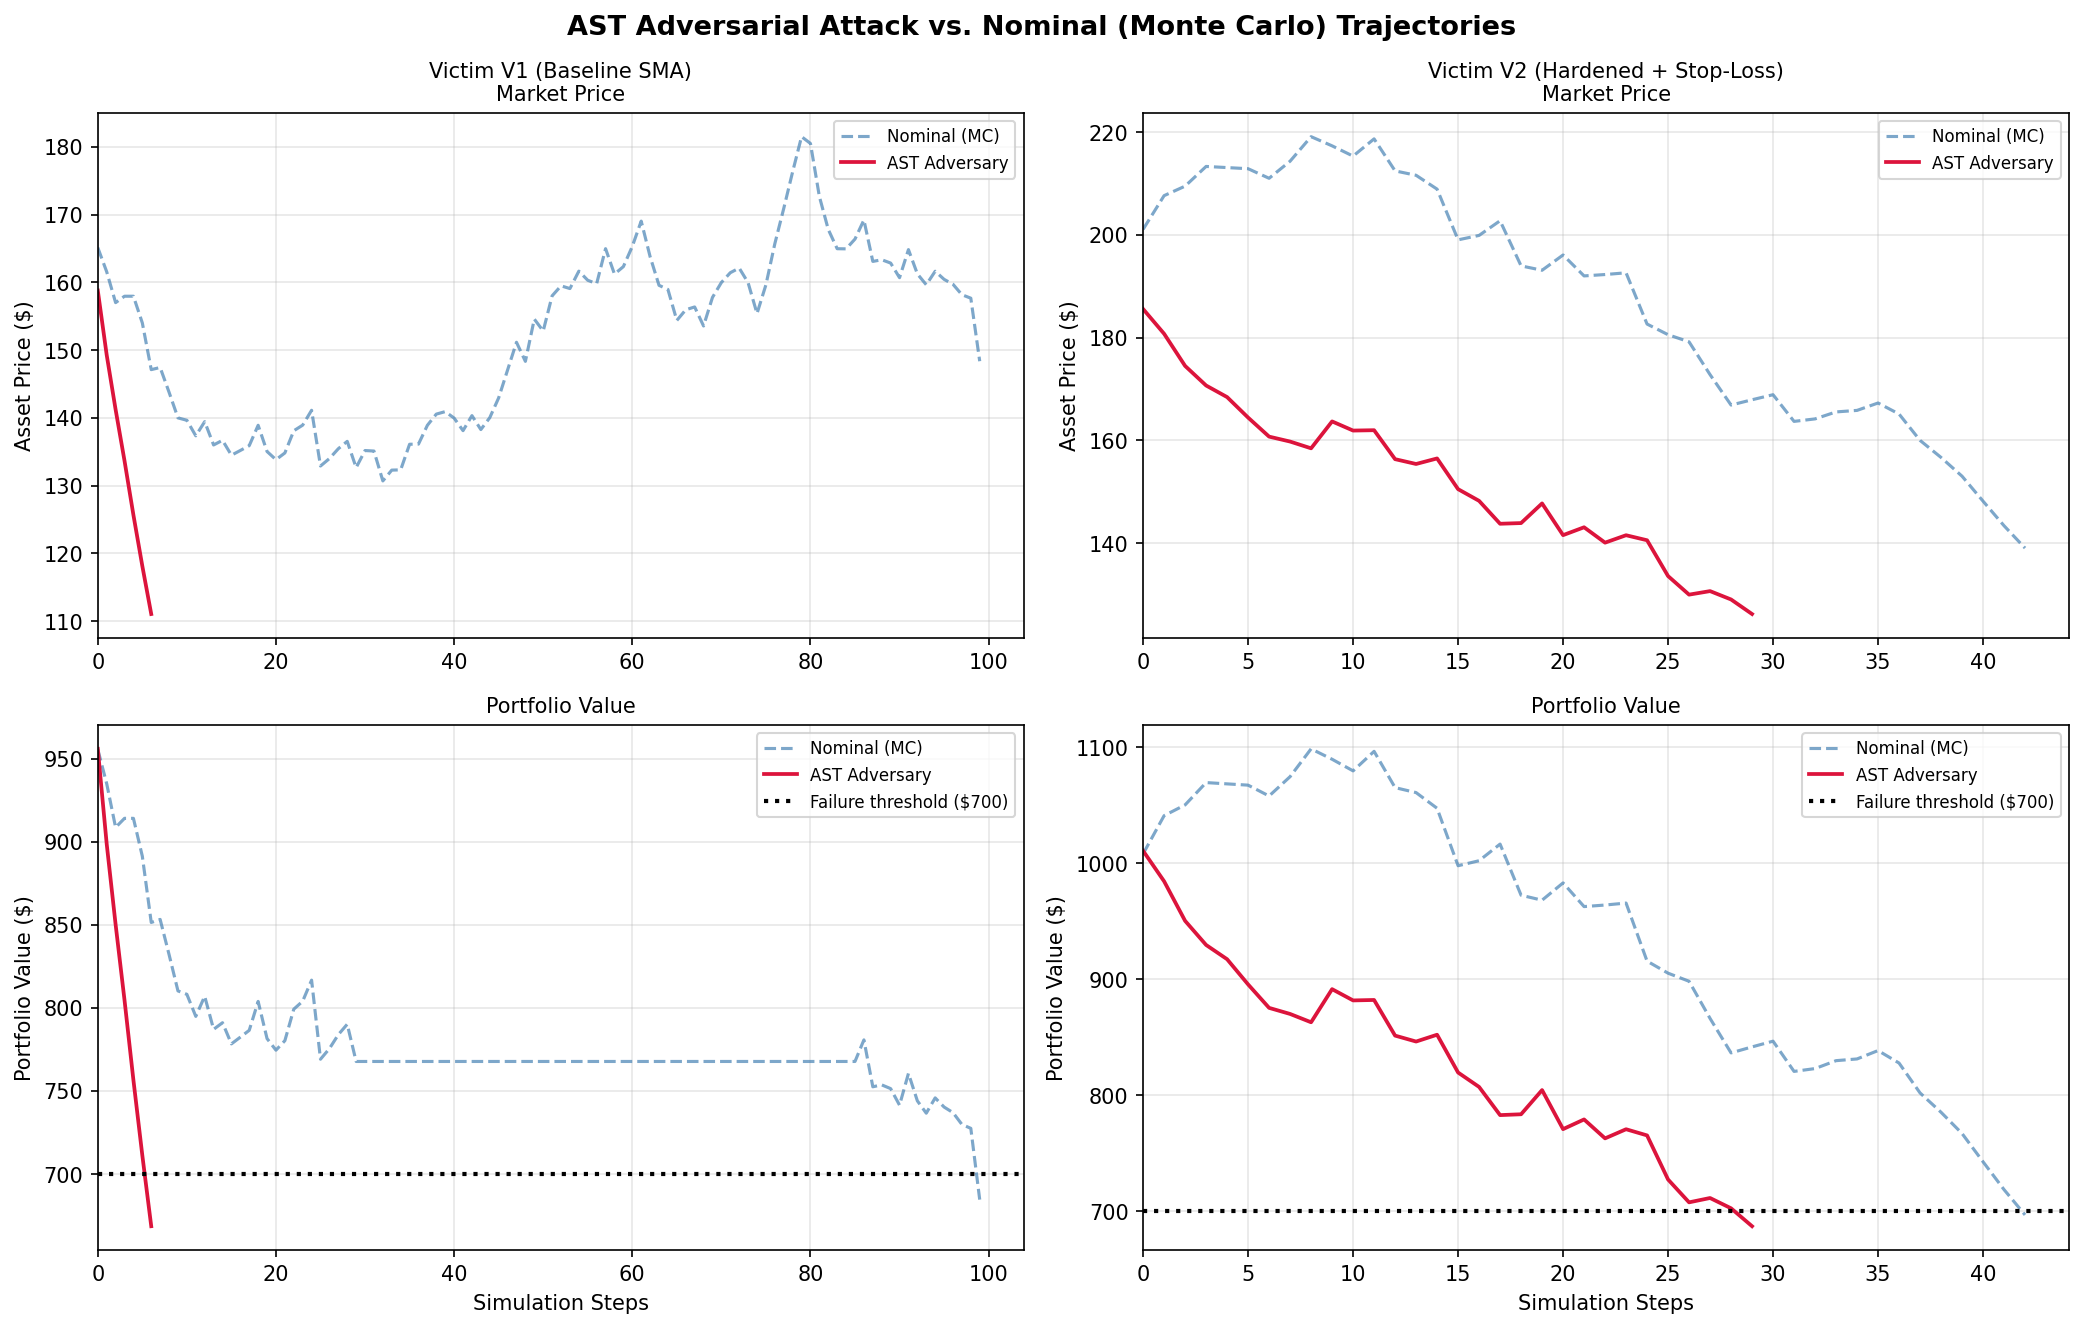
\includegraphics[width=\columnwidth]{results/figure1_trajectories.png}
\caption{Representative market price (top) and portfolio value (bottom) trajectories
for adversarial AST (red) and nominal Monte Carlo (blue) conditions, for both
the baseline V1 victim (left) and more robust V2 victim (right). The dashed
horizontal line marks the \$700 failure threshold.}
\label{fig:trajectories}
\end{figure}

\begin{figure}[htbp]
\centering
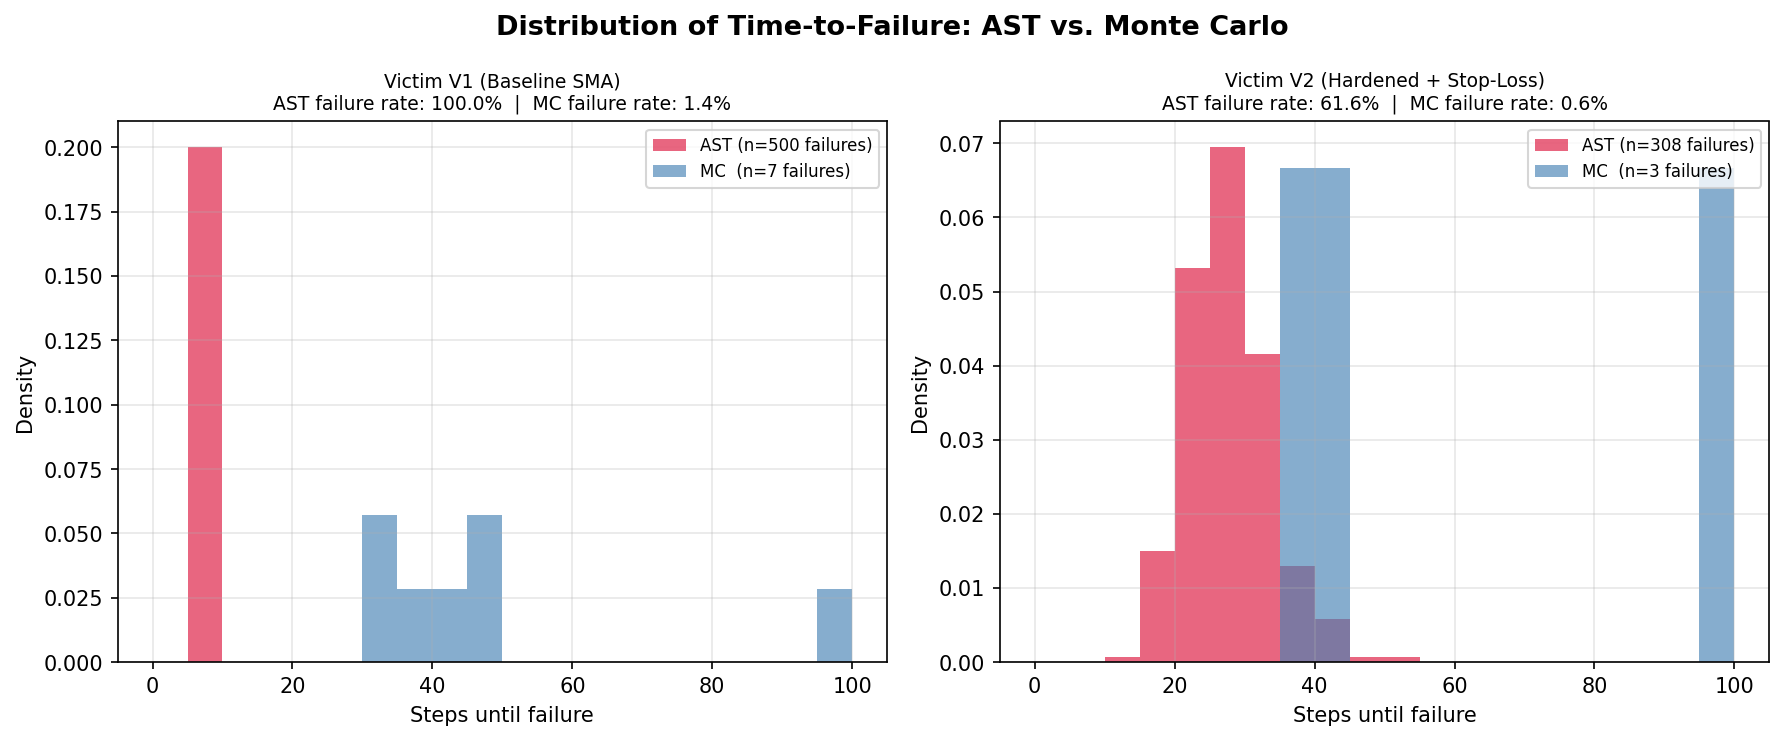
\includegraphics[width=\columnwidth]{results/figure2_failure_histogram.png}
\caption{Distribution of time-to-failure steps, conditioned on episodes
where a failure occurred, for AST (red) and Monte Carlo (blue).
V1+AST failures cluster sharply around 5--10 steps (mean $6.8 \pm 0.0$);
V1+MC failures occur much later (mean $51.5 \pm 20.7$ steps) and are rare
($0.4 \pm 0.3\%$). V2+AST failures ($62.0 \pm 2.6\%$ rate) are spread
across a wider range with a mean of $26.3 \pm 0.3$ steps, reflecting the
longer, more nuanced attack sequence the adversary must discover against
the more robust strategy.}
\label{fig:histogram}
\end{figure}

\subsection{Analysis}

\textbf{AST vs.\ Monte Carlo efficiency.}
Against V1, AST achieves $100.0 \pm 0.0\%$ failure rate across all trials,
while MC achieves only $0.4 \pm 0.3\%$. This corresponds to a
$\geq\!250\times$ improvement in failure discovery efficiency.
The difference in average time-to-failure is equally striking: AST induces
failure in a mean of $6.8 \pm 0.0$ steps, while MC-found failures occur at a
mean of $51.5 \pm 20.7$ steps. This indicates the adversary has learned a
precise and quick-acting attack that exploits the V1 bot's 5-step exit lag:
it delivers a rapid succession of large negative returns before the
SMA crossover signal can trigger an exit.

\textbf{Adversarial sample complexity of V2.}
Against the more robust V2 strategy, the adversary trained for twice the
compute budget (400k vs.\ 200k timesteps) achieves only $62.0 \pm 2.6\%$ failure rate,
compared to $100.0\%$ against V1. The average time-to-failure nearly
quadruples to $26.3 \pm 0.3$ steps, and the average minimum portfolio
value (\$705 vs.\ \$678) is closer to the threshold, indicating the
adversary is barely succeeding.
This demonstrates that the 3-step exit lag forces the adversary to discover
a longer, more nuanced attack sequence that requires significantly more
training timesteps to reliably produce.

\textbf{Importance sampling interpretation.}
The IS-corrected probabilities reveal a striking reversal of intuition.
For V1, $\hat{P}_0(\text{failure}) \approx 1.5 \times 10^{-11}$
($\pm 7.7 \times 10^{-12}$): these failures require extremely non-nominal
actions (avg NLL $4.868 \pm 0.012$ vs.\ $1.420 \pm 0.005$ for MC),
corresponding to sustained ${\approx}3\sigma$ market moves that are
astronomically rare in practice. For V2, however,
$\hat{P}_0(\text{failure}) \approx 2.0 \times 10^{-3}$
($\pm 3.4 \times 10^{-4}$),more than eight orders of magnitude higher.
V2's failures, while harder to find adversarially, occur through more
moderate and realistic market sequences (avg NLL $1.561 \pm 0.005$, only
slightly above the nominal $1.420 \pm 0.005$). This means that although V2
appears more robust by failure rate, its \emph{found} failures are far more
concerning from a real-world safety perspective. IS is essential here: a
naive failure rate comparison ($100.0\%$ vs.\ $62.0\%$) would incorrectly
suggest V2 is safer, while the IS-corrected picture is more nuanced.

% ============================================================
\section{Discussion and Conclusion}

We have demonstrated that Adaptive Stress Testing with importance-sampled
failure probability estimation is an effective framework for the safety
validation of algorithmic trading strategies.

The core advantage of AST over Monte Carlo is computational efficiency:
AST finds failures $\geq\!250\times$ more often than random sampling against
V1 ($100.0\%$ vs.\ $0.4 \pm 0.3\%$), enabling rigorous characterization
of failure modes within a practical compute budget. However, AST failure
rate alone is an incomplete safety metric. V1 appears more dangerous by
failure rate ($100.0\%$ vs.\ $62.0 \pm 2.6\%$), yet IS reveals V2's found
failures are more than eight orders of magnitude more likely to occur
naturally ($2.0\!\times\!10^{-3}$ vs.\ $1.5\!\times\!10^{-11}$).
The IS step is therefore mandatory for converting
adversarial findings into meaningful safety statements.

The iterative robustness improvement experiment illustrates a practical validation
workflow: AST identifies the specific mechanism by which V1 fails
(exploitation of exit lag via rapid quick-acting crashes), which directly
motivates the V2 design choice (reduced exit lag from 5 to 3 steps).
The subsequent AST evaluation of V2 reveals both that V2 is harder to
adversarially exploit and that its residual failures are far more
realistic under the nominal distribution
($2.0\!\times\!10^{-3}$ vs.\ $1.5\!\times\!10^{-11}$). This pairing
of adversarial sample complexity and IS-corrected probability is a more
nuanced safety certificate than either metric alone could provide.

\textbf{Limitations.}
The simulation model is simplified: asset price dynamics follow a
single-asset, constant-volatility model, and the victim strategy does
not incorporate transaction costs, slippage, or portfolio-level risk
constraints. The 100-step episode horizon limits the adversary's ability
to execute longer-horizon manipulation strategies. A further limitation
concerns the nominal distribution itself: we model market noise as
$\varepsilon_t \sim \mathcal{N}(0,1)$, which simplifies the importance
sampling math but does not reflect the well-documented fat-tailed nature
of real financial returns~\cite{cont2001empirical}. In practice, $3\sigma$
events occur far more frequently than a Gaussian predicts, meaning our
IS-estimated probabilities may underestimate true real-world failure
likelihoods for V1 and overstate the rarity of such events. Future work
should replace $\mathcal{N}(0,1)$ with a heavier-tailed nominal
distribution---such as a Student's $t$-distribution or a nonparametric
kernel density estimate fitted to historical log-returns---to produce
more calibrated failure probability estimates. Future work could also
extend the framework to multi-asset portfolios, more realistic
microstructure models, and victim strategies with learned (RL-based)
policies, which would introduce a more complex adversarial interaction.

\textbf{Conclusion.}
Safety validation of financial systems requires methods that can
efficiently characterize rare but catastrophic failure events. AST,
augmented with importance sampling, provides exactly this: efficient
failure discovery combined with statistically valid probability
estimation under the nominal operating distribution. The iterative
robustness improvement loop of discovering failures, patching the system, and re-validating is
a principled framework for improving robustness. Crucially, our results
show that failure rate alone is an incomplete and potentially misleading
safety certificate: V1 appears more dangerous by raw failure rate
($100.0\%$ vs.\ $62.0 \pm 2.6\%$), yet IS reveals V2's residual failures
are more than eight orders of magnitude more likely to occur under natural
market conditions ($2.0\!\times\!10^{-3}$ vs.\ $1.5\!\times\!10^{-11}$).
The IS step is mandatory for converting adversarial findings
into actionable safety statements about real-world risk.

% ============================================================
\bibliographystyle{IEEEtran}
\bibliography{references}

\end{document}
